%
% prinzip.tex -- 
%
% (c) 2015 Prof Dr Andreas Mueller, Hochschule Rapperswil
%
\section{Grundprinzip numerischer Lösungsverfahren}
\rhead{Grundprinzip}
\begin{figure}
\centering
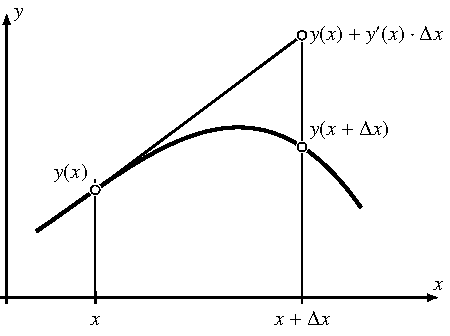
\includegraphics{chapters/50-ode/figures/prinzip.pdf}
\caption{Lineare Approximation von $y(x+\Delta x)$ durch Information,
die am Punkt $x$ verfügbar ist.
\label{buch:ode:lineareapproximation}}
\end{figure}
Wir versuchen als einführendes Beispiel, die Differentialgleichung
\begin{equation}
y'=-\alpha y,\qquad y(0)=y_0
\label{buch:ode:expdgl}
\end{equation}
numerisch zu lösen. 
Die Lösung ist natürlich bekannt, es ist 
\begin{equation}
y(x)=y_0e^{-\alpha x}.
\label{buch:ode:beispiel-loesung}
\end{equation}
Dazu unterteilen wir die $x$-Achse in diskrete Abschnitte der Länge $h$,
genannt die {\em Schrittweite},
\index{Schrittweite}%
und bezeichnen die Teilpunkte mit $x_k=kh$.
Das Ziel ist jetzt, $y(x_k)$ näherungsweise zu berechnen.
Wir schreiben $y_k$ für die Näherungswerte von $y(x_k)$.

Die Ableitung liefert eine lineare Approximation für $y(x)$,
\index{lineare!Approximation}%
\index{Approximation!linear}%
nämlich
\[
y(x+\Delta x)\approx y(x) + y'(x)\cdot\Delta x
\]
(Abbildung~\ref{buch:ode:lineareapproximation}).
Für die Punkte $x_k$ bedeutet das
\[
y(x_{k+1})\approx y(x_{k})+y'(x_k)\cdot h.
\]
Die Differentialgleichung liefert Werte für $y'(x_k)$ aus $x_k$ und $y(x_k)$,
damit können wir aus dieser Approximation ein allgemeines
Näherungsverfahren für die Lösung einer Differentialgleichung
konstruieren.
\index{Näherungsverfahren}%

\begin{satz}[Euler-Verfahren]
\label{buch:satz:euler-verfahren}
\index{Euler-Verfahren}%
Die Differentialgleichung
\begin{equation}
y'=f(x,y),\qquad y(0)=y_0
\label{buch:ode:eulerdgl}
\end{equation}
und die Schrittweite $h$ definieren eine Folge 
\[
y_{\mathstrut k}=y_{k-1} + h\cdot f(x_{k-1}, y_{k-1}),\quad k>0,
\]
mit $x_k=kh$,
die eine Näherung für die Funktionswerte $y(x_k)$ der Lösung $y(x)$
der Differentialgleichung~\eqref{buch:ode:eulerdgl} ist.
\end{satz}

Dieses Verfahren ist nicht besonders gut, wie wir im Folgenden zeigen
wollen.
Die Diskussion soll vor allem zeigen, worauf bei der Weiterentwicklung
des Verfahrens geachtet werden muss.

Im vorliegenden Beispiel liefert die
Differentialgleichung~\eqref{buch:ode:expdgl}
den Wert $y'(x_k)=-\alpha y(x_k)$ für die Ableitung,
woraus wir die Rekursionsformel
\[
y_{k+1}=y_k - \alpha y_k \dot h.
\]
gewinnen.
Die Rekursionsgleichung kann in diesem Fall exakt gelöst werden,
und wir finden
\index{Rekursionsformel}%
\begin{equation}
y(x_{k+1}) = y(x_k)-\alpha y(x_k) h=(1-\alpha h) y(x_k)=\dots
=(1-\alpha h)^{k+1}y_0
\label{buch:ode:rekursion}
\end{equation}
für die Näherung $y_k$ der Funktionswerte $y(x_k)$.

Wir möchten $y(x)$ für einen ganz bestimmten $x$-Wert berechnen.
Dazu unterteilen wir das Intervall $[0,x]$ in $n$ Teilschritte der
Breite $x/n$, und wenden die Formel~\eqref{buch:ode:rekursion} an:
\[
y(x)=y(x_n)=(1-\alpha h)^n y_0=\biggl(1+\frac{-\alpha x}{n}\biggr)^n y_0.
\]
Für eine grosse Zahl von Teilschritten erhalten wir so tatsächlich die
korrekte Lösung:
\[
\lim_{n\to\infty}y_0\biggl(1+\frac{-\alpha x}n\biggr)^n=y_0 e^{-\alpha x}.
\]
\begin{figure}
\centering
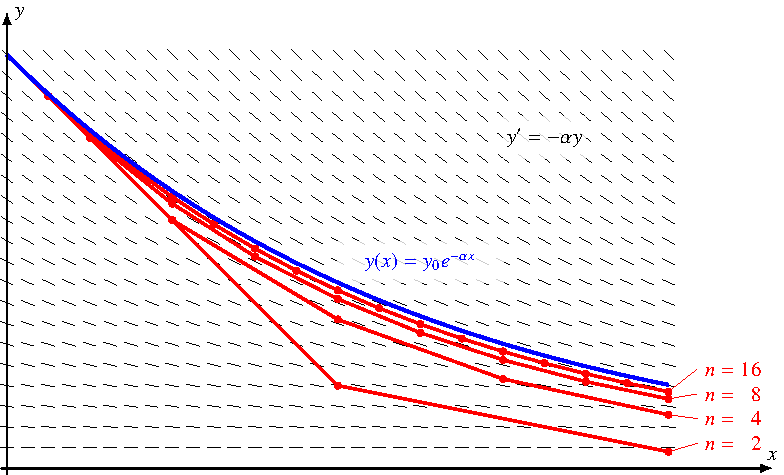
\includegraphics{chapters/50-ode/figures/euler.pdf}
\caption{Approximationen der Lösung der Differentialgleichung $y'=-\alpha y$
mit verschiedener Anzahl Schritte (rot) nähern sich für wachsendes
$n$ der exakten Lösung (blau).
\label{buch:ode:approximation}}
\end{figure}%
Abbildung~\ref{buch:ode:approximation} zeigt, wie die
durch~\eqref{buch:ode:rekursion} gegebenen Approximationen mit zunehmendem
$n$ der exakten Lösung $y(x)=e^{-\alpha x}$ näher kommen.

Wir können auch den Fehler des numerischen Verfahrens berechnen.
Bei der Schrittweite $h$ ist der Fehler von $y_k$ die Differenz
\[
y(x_k)-y_k
=
y_0e^{-\alpha kh}-y_0(1-\alpha h)^k
=
y_0((e^{-\alpha h})^k - (1-\alpha h)^k)
=
y_0e^{-\alpha hk}\biggl(
1-\biggl(\frac{1-\alpha h}{e^{-\alpha h}}\biggr)^k
\biggr).
\]
Man beachte, dass der Zähler $1-\alpha h$ die Approximation
$y_1$ ist, als eine Approximation von $e^{-\alpha h}$, dem Nenner.
Schreiben wir
\[
q=\frac{1-\alpha h}{e^{-\alpha h}},
\]
für den Quotienten zwischen der Approximation und dem korrekten Wert,
dann ist sicher immer $q<1$.
Den Fehler können wir jetzt schreiben
\[
y(x_k)-y_k = y_0e^{-\alpha hk}(1-q^k) = y(x_k)(1-q^k).
\]
Der relative Fehler des Verfahrens ist also
\[
\frac{y(x_k)-y_k}{y(x_k)}=(1-q^k).
\]
\begin{figure}
\centering
%\includegraphics{chapters/images/numerik-3.pdf}
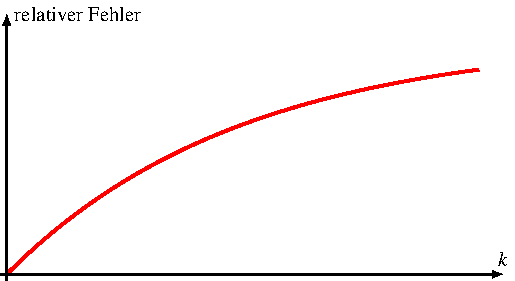
\includegraphics{chapters/50-ode/figures/relativ.pdf}
\caption{Relativer Fehler des Euler-Verfahrens für die Differentialgleichung
\eqref{buch:ode:expdgl} in Abhängigkeit von der Anzahl $k$ der Schritte.
\index{relativer Fehler}%
\label{buch:ode:relfehler}}
\end{figure}%
Ganz unabhängig von der Schrittweite $h$ wird der relative Fehler
des Verfahrens immer gegen 1 streben, der Fehler wird also von der
gleichen Grössenordnung wie die berechneten Resultate.
\index{Schrittweite}%

Die Abbildung~\ref{buch:ode:relfehler} zeigt, dass zu Beginn des Verfahrens
der relative Fehler ungefähr linear mit der Anzahl der Schritte zunimmt.
Um eine angemessene Genauigkeit über einen grösseren Bereich
zu erreichen, muss das Euler-Verfahren also sehr viel kleinere Schritte
und eine entsprechend grössere Anzahl von Schritten ausführen,
die viel Rechenzeit benötigen.
\index{Euler-Verfahren}%

Ein praktisch nützliches Verfahren muss also anstreben, mit einer
sehr viel kleineren Anzahl von Schritten eine deutlich grössere Genauigkeit
der Approximation zu erreichen.



